\graphicspath{ {imgs/} }
\documentclass[main.tex]{subfiles}
\begin{document}
\chapter{Bandit AB-Testing}
\section{Basic Idea}
The previous chapter dealt with optimization concerning classical AB-Testing. The following will describe a fundamentally different approach in which there is no separation between the exploration and the exploitation phase. This is motivated by the idea that valuable costumers could be lost during exploration. Basically this means that we want to already maximize our profit while gaining information about the other buckets. When combining exploration and exploitation one has to chooce on each step if a known good bucket should be used again or if one invests in other unknown buckets to gain more information about their reward function. This balancing is at the core of the now described algorithms.

\subsection{Bandit Algorithms in general}
Bandit algorithms originate from Machine Learning where they serve learning agents to show sensible behavior while exploring the environment. In each time step an agent is forced to make a choice among several actions. An action will lead to a reward. The reward function for any action is not known from the beginning and the agent can only estimate the true reward function of any action by trying this action. The objective is of course to maximize the received reward over the whole experiment. The name of this class of algorithms stems from their relation to the famouse casino slot machines. Each action can be imagined as one lever in a row of many one-armed bandits. Each machine has a hidden reward function and a player wants to maximize their earned money at the end of the evening. The update rule for each step can be roughly formulized as:
\begin{align*}
NewEstimate \leftarrow OldEstimate + StepSize[Target - OldEstimate]
\end{align*}
A K-armed bandit problem is defined by random variables $X_{i,n}$ for $1 \leq i \leq K$ and $n\geq1$ where each $i$ is the index of a slot machine. Successive plays of machine i yield reward $X_{i,1},X_{i,2},...$ which are independent and identically distributed according to an unknown law with unknown expectation $\mu_i$. The machines are also independent.

\subsection{Reformulating AB-Testing to Bandits}
Each new user is our chance to either explore or exploit what we know about the buckets of the test. Each assignment becomes the pull on the lever. The assignments are also independent and identically distributed. We do not know when or if at all the user's behavior will lead to the recording of an action. We will have to assign users before getting the feedback of our previous assignments which leads to a class of bandit algorithms that is concerned with \emph{delayed feedback}. We deal with a stationary environment which means our $StepSize$ is $\frac{1}{k}$ where $k$ denotes the number of assignments. Since we use no prior knowledge there is also \emph{no side information}. 
\subsubsection{Terms}
We want to find the real distributions underlying the variations we made in the buckets. Assume this distributions to be of the form $P_B(y|w)$ where $w$ are the unknown parameters that describe the distribution. By assigning users we generate random observations $D_B=(y_1,y_2..y_t)$.

\subsection{Bandit algorithms}
\subsubsection{epsilon-greedy}
One of the simplest algorithms exploits always the best performing bucket (with the highest conversion rate) exept for $\epsilon $'s fraction of cases where the next bucket is choosen uniformily. For example: if $\epsilon = 0.1$ every tenth assignment would not be to the best performing bucket. This also means that even after convergence for the bucket probabilities $10\%$ of the assignments would not always hit the optimal bucket. For $n$ buckets this would be:
\begin{align*}
P(exploration) \cdot P(\neg best machine | exploration) = \epsilon \cdot \frac{n-1}{n}
\end{align*}
A simulation with 1000 times 1000 assignments gives the following plot for this algorithm:
\begin{figure}[ht]
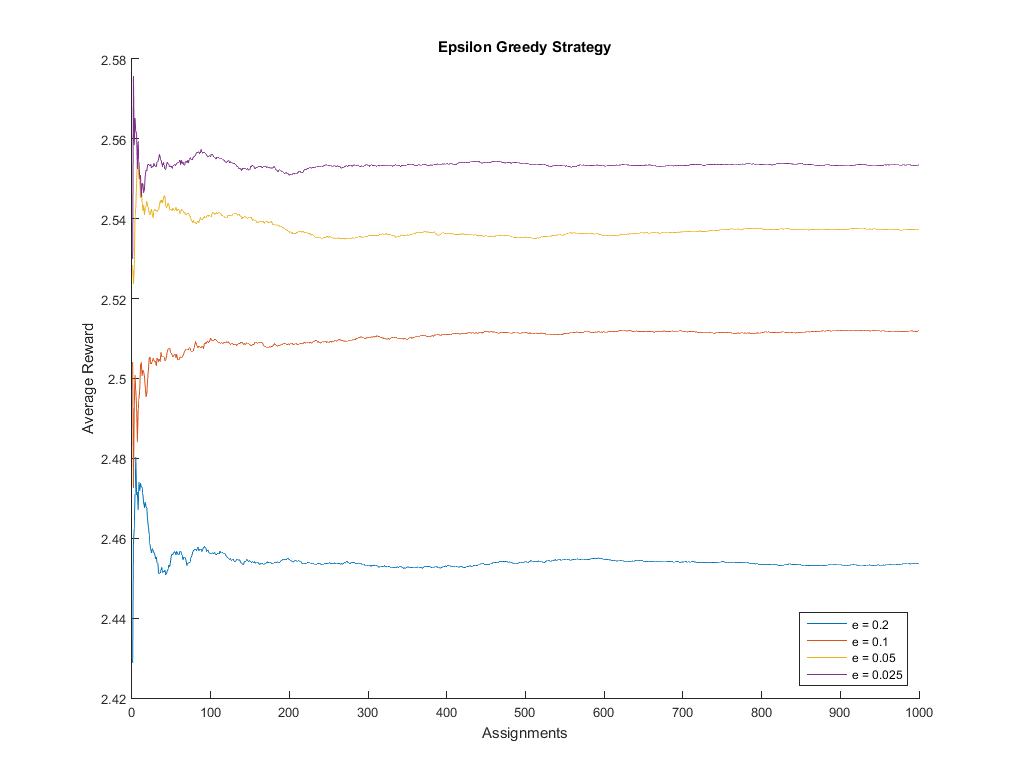
\includegraphics[scale=0.5]{epsGreedy.png}
\centering
\title{Epsilon Greedy}
\end{figure}
\subsubsection{epsilon-first}
Another algorithm that is also basically used by Visual Website Optimizer is called the $\epsilon-first$ algorithm. This is close to A/B-Testing since the exploration phase proceeds the exploitation phase for a finite number of steps and afterwards just exploit.
\begin{figure}[ht]
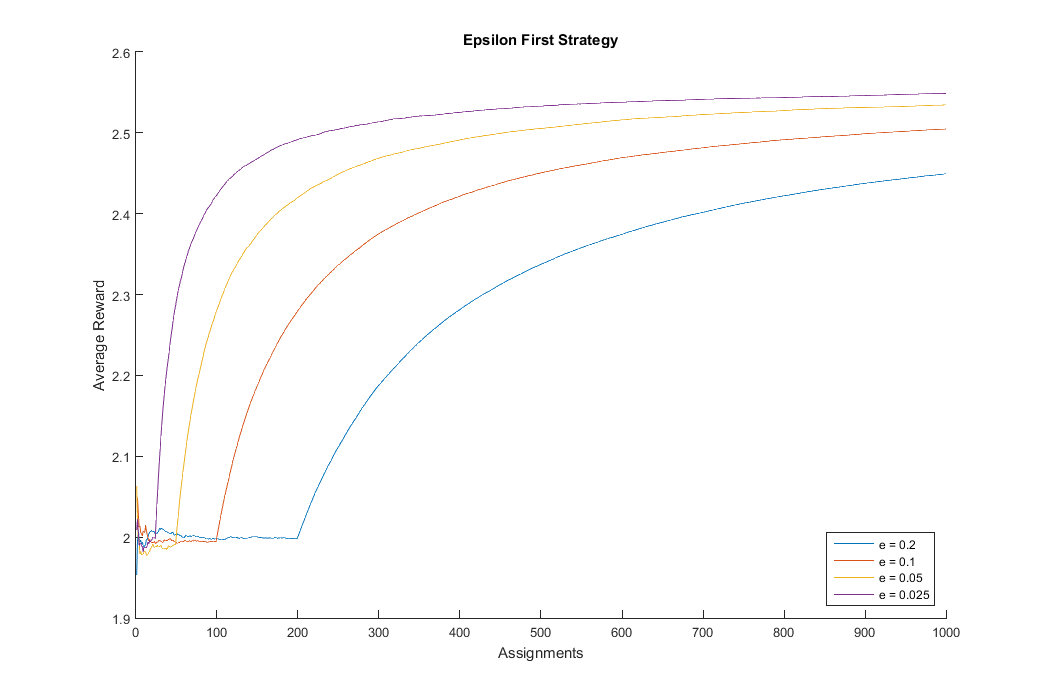
\includegraphics[scale=0.5]{epsFirst.png}
\centering
\title{Epsilon First}
\end{figure}
\subsubsection{UCB}
This algorithm also explores first, but not until a finite number of assignments. The Hoeffding's inequality gives us a confidence bound that models hot sure we are about the estimated payoff across multiple plays. This way - the longer we do not play a machine the more likely it will be played in the future (but only once). The probability for each machine is defined as:
\begin{align*}
mean(b_n) + \sqrt{\frac{2ln(N)}{n_p(b_n)}}
\end{align*}
Here $b_n$ is one of $n$ buckets and $n_p(b_n)$ is the number of times this bucket has been played. $N$ corresponds to the number of assignments across all buckets. This algorithm requirs $mean(b_n)$ to be bounded by 1 so that the confidence bound overpowers the first term. The fraction of time that is spend on exploring decreases exponentially.
\subsubsection{Thompson sampling}
To determine the next bucket to be played, the buckets probability distribution itself is used. They generate numbers that naturally balance between exploitation and exploration, because less performing buckets are demoted and winners promoted by the information already collected.
\subsection{Comparison}
For nearly equal cases some Bandit algorithms need an extra stopping criterion.

\end{document}